\documentclass[tikz,border=5pt]{standalone}
\usetikzlibrary{arrows.meta, calc}

\begin{document}

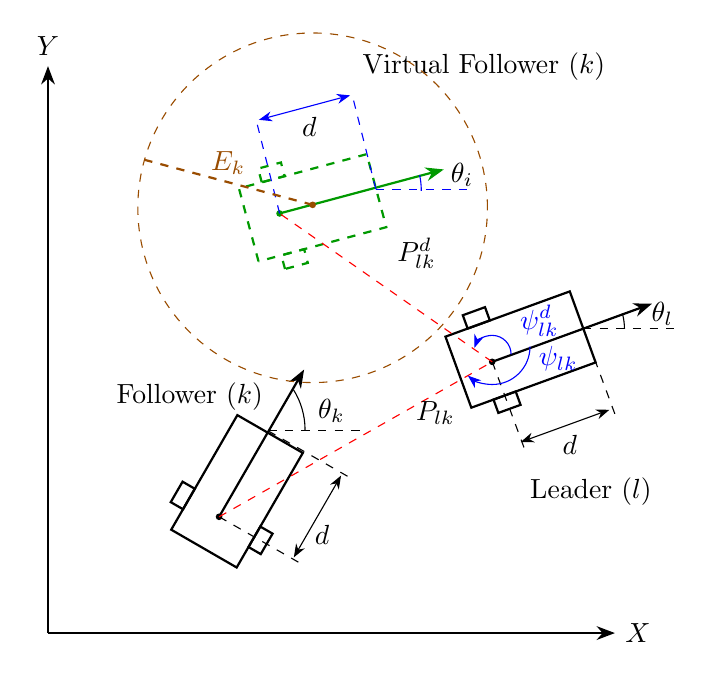
\begin{tikzpicture}[>=Stealth, scale=1.2]
\def\arrowlen{1.8} % độ dài mũi tên
\def\thetak{60} % góc của robot
\def\thetai{15} % góc của robot
\def\wheeloffset{-0.25}
\def\ddiff{1.85}        % giá trị (d_i - d_j)

% ================= AXES =================
\draw[->, thick] (0,0) -- (6,0) node[right] {$X$};
\draw[->, thick] (0,0) -- (0,6) node[above] {$Y$};

% ================= LEADER =================
\coordinate (L) at (5,3);

\begin{scope}[shift={(L)}, rotate=20]
% body
\draw[thick] (-0.7,-0.4) rectangle (0.7,0.4);

% RECTANGULAR SIDE WHEELS
\draw[thick] (-0.45,-0.55) rectangle (-0.2,-0.4); % left wheel
\draw[thick] (-0.45,0.4) rectangle (-0.2,0.55);   % right wheel
\end{scope}

% vector song song thân xe (theo góc 20 độ)
\draw[->, thick] 
($(L)+(-0.3,-0.13)$) -- ++({\arrowlen*cos(20)},{\arrowlen*sin(20)});

% điểm đầu mũi tên
\coordinate (Lhead) at 
($(L)+(-1.03,-0.39)+({\arrowlen*cos(20)},{\arrowlen*sin(20)})$);

% đường song song Ox
\draw[dashed] (Lhead) -- ++(1,0);

% cung góc theta_l (so với trục Ox)
\draw[-, black] 
($(L)+(0.1,-0.48)+(1,0.7)$) 
arc (0.5:15:0.65);

\node at ($(L)+(1.5,0.38)$) {$\theta_l$};


\fill ($(L)+(-0.3,-0.13)$) circle (1pt);
\node[right] at (5,1.5) {Leader ($l$)};

% ====== TÂM TRỤC BÁNH ======
\coordinate (C1) at ($(L)+(-0.3,-0.13)$);

% ====== TỪ TÂM BÁNH ======
\draw[dashed]
let 
    \p1 = (C1),
    \p2 = (Lhead)
in
(\x1,\y1)
--
({\x1 + 1*(\y2-\y1)}, {\y1 - 1*(\x2-\x1)});

% ====== TỪ ĐẦU ROBOT ======
\draw[dashed]
let 
    \p1 = (C1),
    \p2 = (Lhead)
in
(\x2,\y2)
--
({\x2 + 1*(\y2-\y1)}, {\y2 - 1*(\x2-\x1)});

% ================= FOLLOWER =================
\coordinate (F) at (2,1.5);

\begin{scope}[shift={(F)}, rotate=\thetak]
\draw[thick] (-0.7,-0.4) rectangle (0.7,0.4);

% RECTANGULAR SIDE WHEELS
\draw[thick] (-0.45,-0.55) rectangle (-0.2,-0.4); % left wheel
\draw[thick] (-0.45,0.4) rectangle (-0.2,0.55);   % right wheel
\end{scope}

%\draw[->, thick] (F) -- ++(0.8,0.6) node[right] {$\theta_k$};
\draw[->, thick] 
($(F)+(-0.19,-0.27)$) -- ++({\arrowlen*cos(\thetak)},{\arrowlen*sin(\thetak)});

% điểm đầu mũi tên
\coordinate (Lhead) at 
($(F)+(-0.57,-0.92)+({\arrowlen*cos(\thetak)},{\arrowlen*sin(\thetak)})$);

% đường song song Ox
\draw[dashed] (Lhead) -- ++(1,0);

% cung góc theta_l (so với trục Ox)
\draw[-, black] 
($(F)+(0.2,-0.45)+(0.52,1.1)$) 
arc (0:32:0.8);

\node at ($(F)+(1.0,0.85)$) {$\theta_k$};
\fill ($(F)+(-0.19,-0.27)$) circle (1pt);
\node at (1.5,2.5) {Follower ($k$)};

% ====== TÂM TRỤC BÁNH ======
\coordinate (C2) at ($(F)+(-0.19,-0.27)$);

% ====== TỪ TÂM BÁNH ======
\draw[dashed]
let 
    \p1 = (C2),
    \p2 = (Lhead)
in
(\x1,\y1)
--
({\x1 + 1*(\y2-\y1)}, {\y1 - 1*(\x2-\x1)});

% ====== TỪ ĐẦU ROBOT ======
\draw[dashed]
let 
    \p1 = (C2),
    \p2 = (Lhead)
in
(\x2,\y2)
--
({\x2 + 1*(\y2-\y1)}, {\y2 - 1*(\x2-\x1)});
% ================= VIRTUAL FOLLOWER =================
\coordinate (V) at (2.8,4.5);

\begin{scope}[shift={(V)}, rotate=15]
\draw[thick, dashed, green!60!black] (-0.7,-0.4) rectangle (0.7,0.4);

% ONLY 2 REAR WHEELS
\draw[thick, dashed, green!60!black] (-0.45,-0.55) rectangle (-0.2,-0.4);
\draw[thick, dashed, green!60!black] (-0.45,0.4) rectangle (-0.2,0.55);
\end{scope}

\draw[->, thick, green!60!black] ($(V)+(-0.35,-0.06)$) -- ++({\arrowlen*cos(15)},{\arrowlen*sin(15)});

% điểm đầu mũi tên
\coordinate (Lhead) at 
($(V)+(-1.07,-0.27)+({\arrowlen*cos(15)},{\arrowlen*sin(15)})$);

% đường song song Ox
\draw[dashed, blue] (Lhead) -- ++(1,0);

% cung góc theta_i (so với trục Ox)
\draw[-, blue] 
($(V)+(0.2,-0.48)+(0.95,0.66)$) 
arc (0:12:0.8);

\node at ($(V)+(1.58,0.35)$) {$\theta_i$};
\fill[green!60!black] ($(V)+(-0.35,-0.06)$) circle (1pt);
\node[left] at (6,6) {Virtual Follower ($k$)};

% ====== TÂM TRỤC BÁNH ======
\coordinate (C3) at ($(V)+(-0.35,-0.06)$);

% ====== TỪ TÂM BÁNH ======
\draw[dashed, blue]
let 
    \p1 = (C3),
    \p2 = (Lhead)
in
(\x1,\y1)
--
({\x1 - 1*(\y2-\y1)}, {\y1 + 1*(\x2-\x1)});

% ====== TỪ ĐẦU ROBOT ======
\draw[dashed, blue]
let 
    \p1 = (C3),
    \p2 = (Lhead)
in
(\x2,\y2)
--
({\x2 - 1*(\y2-\y1)}, {\y2 + 1*(\x2-\x1)});

\draw[dashed, orange!60!black] (V) circle (1.85);
% ====== TÂM TRỤC BÁNH VIRTUAL FOLLOWER ======
\coordinate (Vc) at ($(V)+(0,0.03)$);

% ====== VẼ CHẤM TRÒN ======
\fill[orange!60!black] (Vc) circle (1pt);

% ====== VẼ ĐOẠN (d_i - d_j) ======
\draw[-, thick, dashed, orange!60!black]
(Vc) -- ++({\ddiff*cos(180-\thetai)},{\ddiff*sin(\thetai)});

% ====== LABEL ======
\node[orange!60!black] 
at ($(Vc)+({0.5*\ddiff*cos(180-\thetai)},{0.5*\ddiff*sin(\thetai)}) + (0,0.2)$) 
{$E_k$};
% ================= CONNECTION =================
%\draw[dashed, red] (F) -- (L);
%\draw[dashed, red] (L) -- (V);
\draw[dashed, red] 
($(F)+(-0.19,-0.27)$) -- ($(L)+(-0.3,-0.13)$);
\draw[dashed, red] 
($(L)+(-0.3,-0.13)$) -- ($(V)+(-0.35,-0.06)$);

% ================= LABELS =================
\node at ($(F)!0.7!(L)$) [below] {$P_{lk}$};
\node at ($(L)!0.5!(V)$) [above] {$P^d_{lk}$};

% ================= ANGLES =================
\draw[->, blue] ($(L)+(0.1,0.03)$) arc (0:-130:0.4);
\node[blue] at ($(L)+(0.4,-0.1)$) {$\psi_{lk}$};

\draw[->, blue] ($(L)+(-0.1,-0.05)$) arc (0:160:0.2);
\node[blue] at ($(L)+(0.2,0.3)$) {$\psi^d_{lk}$};

% ================= DISTANCE =================
%\draw[<->] ($(L)+(0,-1)$) -- ($(L)+(1,-0.5)$);
%\node at ($(L)+(0.5,-1.1)$) {$d$};
% ====== ĐIỂM BẮT ĐẦU (tâm bánh hoặc gần đó) ======
\coordinate (C1) at ($(L)+(0,-0.98)$);
\def\dlen{1}  % độ dài đoạn d
\def\thetal{20} % góc của robot
% ====== VẼ d SONG SONG ROBOT ======
\draw[<->]
(C1) -- ++({\dlen*cos(20)},{\dlen*sin(20)});

% ====== LABEL d ======
\node at ($(C1)+({0.5*\dlen*cos(\thetal)},{0.5*\dlen*sin(\thetal)}) + (0.05,-0.2)$) {$d$};

%\draw[<->] ($(F)+(-0.8,-0.3)$) -- ($(F)+(-1.6,-0.8)$);
%\node at ($(F)+(-1.2,-0.9)$) {$d$};
% ====== ĐIỂM BẮT ĐẦU (tâm bánh hoặc gần đó) ======
\coordinate (C2) at ($(L)+(-2.4,-2.2)$);
%\def\dlen{1}  % độ dài đoạn d

% ====== VẼ d SONG SONG ROBOT ======
\draw[<->]
(C2) -- ++({\dlen*cos(\thetak)},{\dlen*sin(\thetak)});

% ====== LABEL d ======
\node at ($(C2)+({0.5*\dlen*cos(\thetak)},{0.5*\dlen*sin(\thetak)}) + (0.05,-0.2)$) {$d$};

%\draw[<->, green!60!black] ($(V)+(-0.6,0.6)$) -- ($(V)+(-1.4,1.1)$);

%\node[green!60!black] at ($(V)+(-1,1.2)$) {$d$};
% ====== ĐIỂM BẮT ĐẦU (tâm bánh hoặc gần đó) ======
\coordinate (C3) at ($(L)+(-2.77,2.43)$);
%\def\dlen{1}  % độ dài đoạn d
% ====== VẼ d SONG SONG ROBOT ======
\draw[<->, blue]
(C3) -- ++({\dlen*cos(\thetai)},{\dlen*sin(\thetai)});

% ====== LABEL d ======
\node at ($(C3)+({0.5*\dlen*cos(\thetai)},{0.5*\dlen*sin(\thetai)}) + (0.05,-0.2)$) {$d$};
\end{tikzpicture}

\end{document}